\documentclass{report}
\usepackage[T1]{fontenc} % Fontes T1
\usepackage[utf8]{inputenc} % Input UTF8
\usepackage[backend=biber, style=ieee]{biblatex} % para usar bibliografia
\usepackage{csquotes}
\usepackage[portuguese]{babel} %Usar língua portuguesa
\usepackage{blindtext} % Gerar texto automaticamente
\usepackage[printonlyused]{acronym}
\usepackage{hyperref} % para autoref
\usepackage{graphicx}
\usepackage{indentfirst}
\usepackage{pgfplots}
\usepackage{url}
\usepackage{pgf-pie}
\usepackage{float}

\bibliography{bibliografia.bib}

\begin{document}
%%
% Definições
%
\def\titulo{CIBERCRIMINALIDADE \\ \Large os casos mais impactantes}
\def\data{DATA}
\def\autores{Joana Gião, Matilde Sanches}
\def\autorescontactos{126489 joanagiao@ua.pt, 125369 matilde.sanches@ua.pt}
\def\versao{VERSAO 1}
\def\departamento{Dept. de Eletrónica, Telecomunicações e Informática}
\def\empresa{Universidade de Aveiro}
\def\logotipo{imagens/ua.pdf}
\def\repo{infor2024-ap-52}
%
%%%%%% CAPA %%%%%%
%
\begin{titlepage}

\begin{center}
%
\vspace*{50mm}
%
{\Huge \titulo}\\ 
%
\vspace{10mm}
%
{\Large \empresa}\\
%
\vspace{10mm}
%
{\LARGE \autores}\\ 
%
\vspace{30mm}
%
\begin{figure}[h]
\center
\includegraphics{\logotipo}
\end{figure}
%
\vspace{30mm}
\end{center}
%
\begin{flushright}
\versao
\end{flushright}
\end{titlepage}

%%  Página de Título %%
\title{%
{\Huge\textbf{\titulo}}\\
{\Large \departamento\\ \empresa}
}
%
\author{%
    \autores \\
    \autorescontactos
}
%
\date{\today}
%
\maketitle

\pagenumbering{roman}

%%%%%% RESUMO %%%%%%
\begin{abstract}

Nesta era digital, é quase impossível não ter sido vítima de, pelo menos, uma tentativa de ataque cibernético. Estes ataques tornaram-se muito comuns porque a internet possibilitou algo que todos os criminosos desejavam, "uma nova identidade". Ou seja, um criminoso pode muito bem cometer crimes e nunca ser apanhado pelos mesmos. É destes casos e mais que este relatório se focou. \\ \indent Deste modo, este trabalho tem como objetivo analisar o impacto que o cibercrime consegue ter no mundo e abordar a importância da cibersegurança, a única solução para este tipo de ataque. \\ \indent Através de uma análise dos casos apresentados, são explorados os perigos da tecnologia e as suas consequências. Estas consequências indicam que, embora esta melhore a nossa vida quotidiana, também pode ter um impacto muito negativo na mesma se não estivermos devidamente informados. Esta análise também revela que a proteção cibernética é igualmente crucial para as grandes empresas e para utilizadores comuns.\\ \indent
Com isto, conclui-se que a falta de investimento e conhecimento em medidas de segurança aumenta a vulnerabilidade a ataques informáticos. Isto é, empresas bem preparadas, com políticas de segurança atualizadas e bons profissionais na área conseguem reduzir os riscos de maneira mais eficaz.\\\indent

\end{abstract}

\renewcommand{\contentsname}{Índice}
\tableofcontents

%\listoftables     % descomentar se necessário
\listoffigures    % descomentar se necessário


%%%%%%%%%%%%%%%%%%%%%%%%%%%%%%%
\clearpage
\pagenumbering{arabic}

%%%%%%%%%%%%%%%%%%%%%%%%%%%%%%%%
\chapter{Introdução}
\label{chap.introducao}


Como a cibersegurança é algo muito relacionado ao nosso curso, Engenharia de Computadores e Informática, havendo até um mestrado da mesma, é pertinente aprofundar os nossos conhecimentos nesta área. Trata-se de um tema que desperta interesse e que é cada vez mais importante na sociedade atual. \\ \indent Por essas mesmas razões, é oportuno realizar um trabalho que aborde o mesmo e que sensibilize a importância de nos mantermos informados e seguros no âmbito digital. O relatório apresenta o tema de forma indireta, através de uma exposição sobre a cibercriminalidade, apresentando os exemplos que se consideram mais impactantes e envolventes, de modo a compreender as consequências que uma rede insegura pode causar. \\ \indent Para tal, no \autoref{chap.os-crimes}, são abordadas as histórias de vários indivíduos com habilidades informáticas invejáveis, que lhes possibilitaram a cometer crimes maiores do que se esperava. \\ \indent No \autoref{chap.a-solução}, chega-se ao cerne da questão e levanta-se o que poderia ter evitado todos estes crimes, a cibersegurança. \\ \indent Finalmente no \autoref{chap.conclusão}, encontram-se as conclusões que são possíveis retirar com este relatório.

\chapter{Os Crimes}
\label{chap.os-crimes}
Neste capítulo, vamos abordar os acontecimentos mais impactantes de cibercriminalidade até hoje.
\section{O rapaz que roubou milhões de euros com o computador}

O grupo russo de \textit{hackers} “Evil Corp”, é acusado de roubar cerca de 300 milhões de euros em cerca de 10 anos. Alegadamente, o líder desse grupo é o informático, e \textit{hacker}, Maksim Yakubets. Para além de líder deste grupo, o mesmo também é responsável pela conspiração do \textit{malware} nomeado “Bugat”, também conhecido como Dridex ou Cridex. Este malware está programado para roubar as credenciais do banco das vítimos usando, maioritariamente, ataques de “phishing”, ou seja, fingindo ser uma entidade ou pessoa, de modo a fazer a vítima instalar o \textit{malware}. \\ \indent 

\begin{figure}[h]
    \center
    \fbox{
\includegraphics[width=0.5\textwidth]{imagens/evilcorp.png}}
    \caption{Evil Corp}
    \label{evilcorp}
\end{figure}

No mais recente ataque, estes criminosos ligados ao \textit{malware}, mandaram emails a membros do LinkedIn, como se fossem a própria empresa, a alertar de mensagens não lidas, seguido de um link perigoso, no seguimento da abertura deste link, um \textit{java applet}\footnote{java applet é um programa incorporado na página web. Ele funciona tanto dentro do navegador como no lado do cliente.} foi instalado e, assim, o \textit{malware} também o foi. Posteriormente, os \textit{hackers} tiveram acesso a toda a \textit{data} roubada, que, por suas vezes, utilizaram as informações para fraudes, como a "ACH fraud", que consiste em transferências não autorizadas feitas a partir da conta bancária utilizando a rede \ac{ach}, rede que processa pagamentos e transferências eletrónicas nos Estados Unidos e no Canadá. \\ \indent Este \textit{malware}, ao longo do tempo, foi atualizado diversas vezes de modo a ser cada vez mais eficiente. A mais recente e conhecida versão rouba informações sensíveis a quem usa o Firefox e a quem usava o Internet Explorer (antigo Microsoft Edge). Este tipo de roubo costuma acontecer a médias empresas.\\ \indent Para além do envolvimento no Bugat, Maksim Yakubets, também esteve muito envolvido no \textit{malware} Zeus, conhecido também como Zeus Trojan Malware (Malware Cavalo de Troia Zeus), isto porque o mesmo atua como um cavalo de Troia, ou seja, vigia sites e regista as teclas que foram pressionadas no mesmo, para que quando o \textit{malware} perceber que a vítima está no site, guardar as teclas usadas para o login. Desse modo, quebra toda a segurança e consegue aceder à conta da vítima. Conseguindo, assim, roubar municípios, bancos, organizações sem fins lucrativos e uma congregação religiosa, e ganhar cerca de 60 milhões de euros. \cite{osmaisprocurados}  \\ \indent Com estes dois \textit{malwares}, o grupo conseguiu roubar mais de 100 milhões de euros.\\ \indent Ainda, em 2017, o governo norte-americano afirmou que Maksim começou a trabalhar para os serviços secretos russos e que no ano a seguir estava a trabalhar para obter uma licença de aceso a informações confidenciais da mesma.\\ \indent O mais interessante e revoltante desta história é o facto de Maksim Yakubets não precisar de se esconder, aliás, o mesmo exibe de forma exuberante o dinheiro. Na \autoref{lambo} é possível verificar isso mesmo: Maksim com o seu lamborghini modificado, com "BOP" na matrícula, que significa ladrão em russo, a falar com um polícia, como se não fosse nada. Na \autoref{audi} é possível observar um Audi R8, alterado com o mesmo padrão e com a matrícula também alterada. Para além disso teve um casamento que custou cerca de 300 mil euros.
\begin{figure}[h]
\begin{minipage}{0.50\textwidth}
    \center
    \fbox{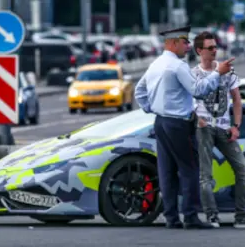
\includegraphics[width=0.49\textwidth]{imagens/maksimyakubetslamborghini.png}}
    \caption{Maksim com polícia e Lamborghini atrás}
    \label{lambo}
\end{minipage}
\begin{minipage}{0.50\textwidth}
    \center	
    \fbox{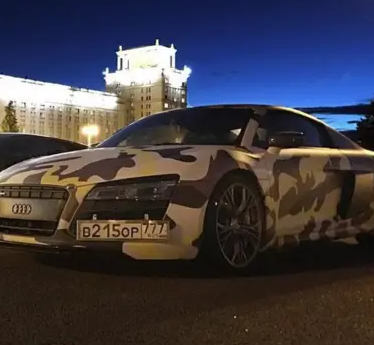
\includegraphics[width=0.49\textwidth]{imagens/audir8.png}}
    \caption{Audi R8 alterado}
    \label{audi}
\end{minipage}
\end{figure}

Isto acontece porque, mesmo com as imensas acusações americanas contra o \textit{hacker} e com a oferta de uma recompensa de 5 milhões de euros a quem fornecesse informações sobre o paradeiro de Yakubets por parte do Departamento de Estado norte-americo \cite{maksimprocurado}, o governo russo ignora as acusações de crimes cibernéticos vindas dos \ac{eua} contra os seus cidadãos. A \ac{nca} continua a garantir que: “Se Maksim Yakubets deixar a segurança da Rússia, será imediatamente detido e extraditado para os Estados Unidos”. Porém, até hoje, parece que o mesmo não aconteceu e Maksim continua em liberdade.

\section{Os adolescentes que hackearam a \ac{cia}}
Em outubro de 2015, John Brennan, um dos homens mais poderosos da Terra, o chefe da \ac{cia}, recebe uma chamada telefónica de um estranho. Isto poderia ter parecido uma brincadeira comum. "Quem é? Como conseguiu este número? O governo dos \ac{eua} classificará esta chamada como parte de uma grande conspiração de roubo de identidade, assédio a funcionários do governo e ciberterrorismo.” O estranho exigiu que parassem de bombardear o Médio Oriente antes de desligar. Um miúdo de 15 anos, no seu quarto, com o telefone ainda na mão, não consegue acreditar no que acabou de fazer. Ele é líder dos Crackers With Attitude, um grupo que aterrorizou e humilhou as organizações secretas do \ac{eua}. 

\begin{figure}[h]
    \center
    \fbox{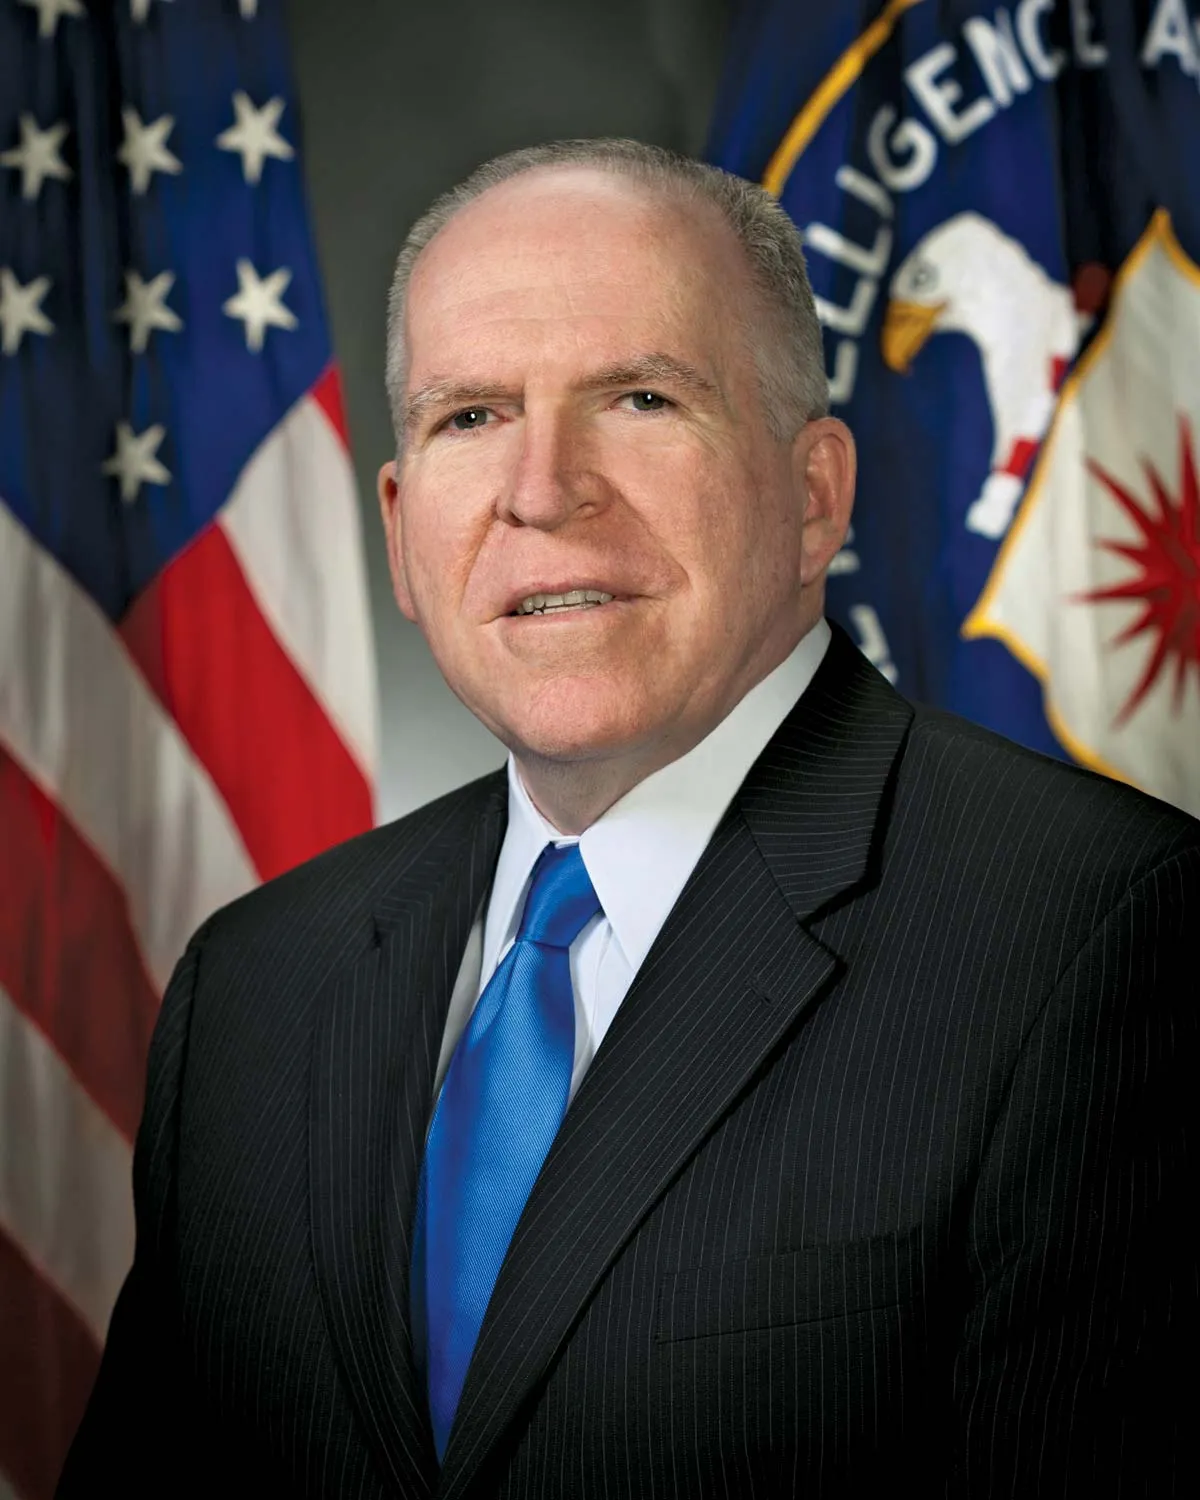
\includegraphics[width=0.5\textwidth]{imagens/johnbrennan.png}}
    \caption{John Brennan}
    \label{johnbrennan}
\end{figure}


Cada vez mais, os \textit{hacks} deste grupo eram motivados pelo altruísmo, em vez da simples curiosidade. Como por exemplo, em 2014, quando a bestialidade era legal na Dinamarca. Outros países europeus, como a Alemanha, o Reino Unido e a Suécia, já a tinham proibido. Isto significou para a Dinamarca um aumento do turismo sexual com animais. Durante anos, os ativistas pelos direitos dos animais na Dinamarca tentaram chamar a atenção para esta situação. Chamavam-lhe "canil de cães". O rapaz, de nome Kraker, tinha um cão e isso irritou-o, levando o grupo a desligar o site oficial do governo dinamarquês e depois desfiguraram-lo. Não só isto, mas também desligaram sites através de ataques de negação de serviço e publicaram no Twitter provas de animais sexualmente maltratados. A informação repercutiu-se em todo o mundo e foi amplamente condenada \cite{adolescentecia}. \\ \indent Enquanto isso, em Virgínia, um rapaz que se autodenomina "default" começou a aprender tudo o que era possível sobre computadores apenas guiado pela curiosidade. Ele ficou impressionado com um grupo chamado Anonymous no início, mas começou a perder o interesse quando entendeu que o grupo estava a crescer astronomicamente, tornando difícil saber em quem confiar. Então, este junta-se ao grupo \textit{krakas with Attitude} unidos pelo ódio que tinham contra o governo americano especialmente com a sua posição no conflito entre Israel e a Palestina. Hackearam documentos confidenciais de membros da Intelligence Comunity conseguindo entrar no email de um dos membros mais importantes da mesma. Em outubro de 2015, o grupo publicou os documentos incluindo o formulário SF-86 de 47 páginas de Brennan, um documento sensível exigido para obter uma autorização de segurança governamental de alto nível. Além disso, a partir dos e-mails de Brennan, o WikiLeaks publicou recomendações da era Bush sobre como a presidência deveria operar no Médio Oriente. \\ \indent Infelizmente, devido a dois deslizes, um dos membros acabou por se entregar ao contar a uma rapariga o que eles faziam enquanto estava bêbado. Consequentemente, Default recebeu uma visita do \ac{fbi} no dia seguinte que encontrou todo o seu equipamento e prendeu-o de imediato. Kraka é também preso pelas forças policiais Inglesas. Default foi condenado a 5 anos de prisão, com uma multa de 145 mil dólares. Atualmente, Kraka deixou a vida de crime e esta atualmente a estudar cibersegurança \cite{presocia}.
\section{A \textit Koobface \textit{Gang}}
No ano de 1997 o website mais popular é o Yahoo! Com mais de 17 milhões de utilizadores ativos por mês a descobrir um novo mundo: a internet. No entanto dia 8 de dezembro ás 7 da noite, o Yahoo é hackeado. Qualquer pessoa que abra o browser terá uma mensagem no seu computador a dizer que todos os computadores que acederam ao Yahoo no mês passado serão destruídos por uma bomba que será detonada no Natal. Isto é, apenas se as exigências dos hackers não forem cumpridas, que se referem a libertar um tal Kevin. E muitos se perguntaram, quem é o Kevin? Ele não é um chefe da máfia ou um assassino, e ele não está na prisão por ter ameaçado agentes dos estados unidos. Este indivíduo é muito mais perigoso do que isto: dizem que com apenas uma chamada telefónica ele consegue entrar e tomar controlo do arsenal nuclear dos EUA.\\ \indent No início, o grupo KoobFace utilizava contas manualmente criadas para espalhar o vírus mas com o crescimento das empresas, estes precisavam de uma maneira de autocriar dezenas de contas falsas que passassem pelas verificações humanas e atrair as suas vítimas. Primeiro, o login e a password são codificadas através de um processo que envolve ler letras e comparar o seu valor AC a uma string de números de 0 a 1, de 2 a 3 a 4 conseguindo assim entrar na plataforma e personalizando o perfil com informações pessoais autogeradas que parecem realistas o suficiente. De seguida, o site pede CAPTCHA. Para circundar isto, o puzzle é espelhado na área de trabalho de qualquer indivíduo do seu exército de bots. Milhões de pedidos de amizade são mandados na rede social Facebook conseguindo infetar cerca de 600 mil máquinas.\\ \indent Um dia, sem qualquer explicação aparente, o controlo de comandos simplesmente fica offline. Desde então o seu centro de controlo original nunca mais foi ativado. Os seus membros continuam por aí, e os vírus dormentes nos computadores infetados.
\\


\begin{figure}[h]
    \center
    \fbox{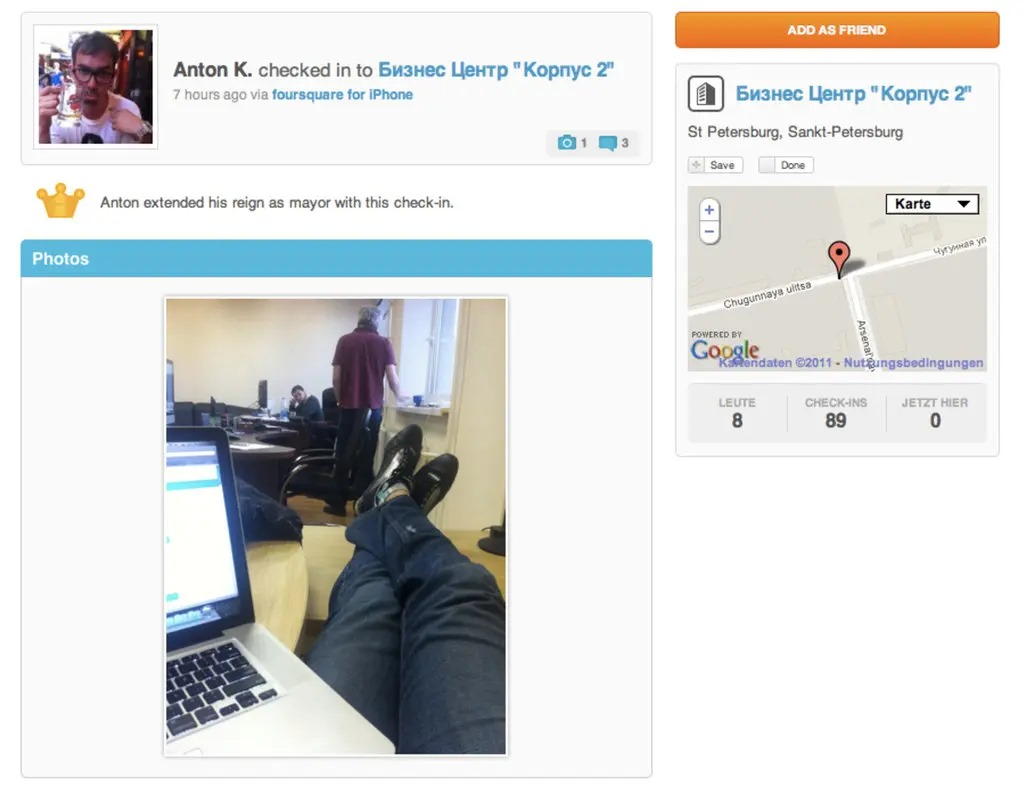
\includegraphics[width=0.5\textwidth]{imagens/koobface.jpg}}
    \caption{Foto publicado por um membro da Koobface que mostra o escritório e as suas coordenadas em St.Petersburg}
    \label{koobface}
\end{figure}
\begin{figure} [h]
    \center
    \fbox{
\includegraphics[width=0.8\textwidth]{imagens/membros.jpg}}
    \caption{Alguns membros da gangue}
    \label{membros}
\end{figure}

Quando criança, Kevin infiltrou-se no sistema dos Estados Unidos por pura diversão. Mais tarde foi apanhado e preso por 12 meses. No entanto no seu julgamento, Kevin mostra as suas incríveis habilidades de manipulação, conseguindo manipular o juíz a libertá-lo mais cedo. O hacker rouba milhares de empresas mas acaba por ser apanhado devido a um deslize. Kevin provocou um hacker de elite que conseguiu descobrir onde este vivia. Este quase conseguiu escapar da situação, mas um dos agentes do FBI encontra um paycheck com o nome dele. É preso por cerca de quatro anos. A noite de Natal passa sem problemas, não há bomba e o site Yahoo voltou ao normal. Quando saiu da prisão, Kevin ajudou o governo a fortalecer a sua segurança digital, tornando-se um “White hacker”.
\\ Informações encontradas num artigo do New York Times \cite{newyorktimes}. 
\section{A criadora da \textit{OneCoin}}
Em 2014, A OneCoin foi criada, uma suposta criptomoeda rival da original Bitcoin, uma grande promessa para retornos gigantes. Esta moeda foi criada por Ruja Ignatova, também conhecida por "rainha das criptomoedas", antiga estudante de Oxford e doutorada em Direito Privado Europeu na Universidade de Kontanz, Alemanha \cite{osmaisprocurados}.
\begin{figure}[h]
    \center
    \fbox{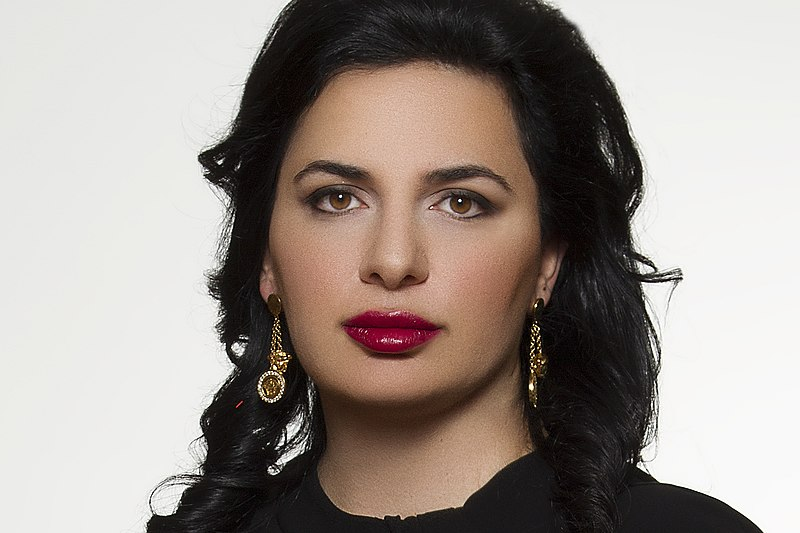
\includegraphics[width=0.5\textwidth]{imagens/rujaignatova.jpg}}
    \caption{Ruja Ignatova}
    \label{rujaignatova}
\end{figure}
\\
A OneCoin foi um sucesso! Ignatova convenceu milhares de investidores de mais 170 países a investirem na moeda através de uma plataforma de cursos online sobre criptomoedas e tokens. Estes tokens eram depois usados para obter as tais OneCoins. Mas na verdade, o que Ruja escondia, era que por trás da moeda, esta totalmente falsa, estava uma fraude de investimento imensa, sem o registro digital subjacente às criptomoedas de facto legítimas, que levou a diversos alertas por parte das autoridades financeiras e bancos nacionais. Mesmo assim, entre 2014 e 2016, Ignatova conseguiu lucrar cerca de 3,5 mil milhões de euros \cite{osmaisprocurados}. \\ \indent
\\
\begin{figure}[h!]
    \center
    \fbox{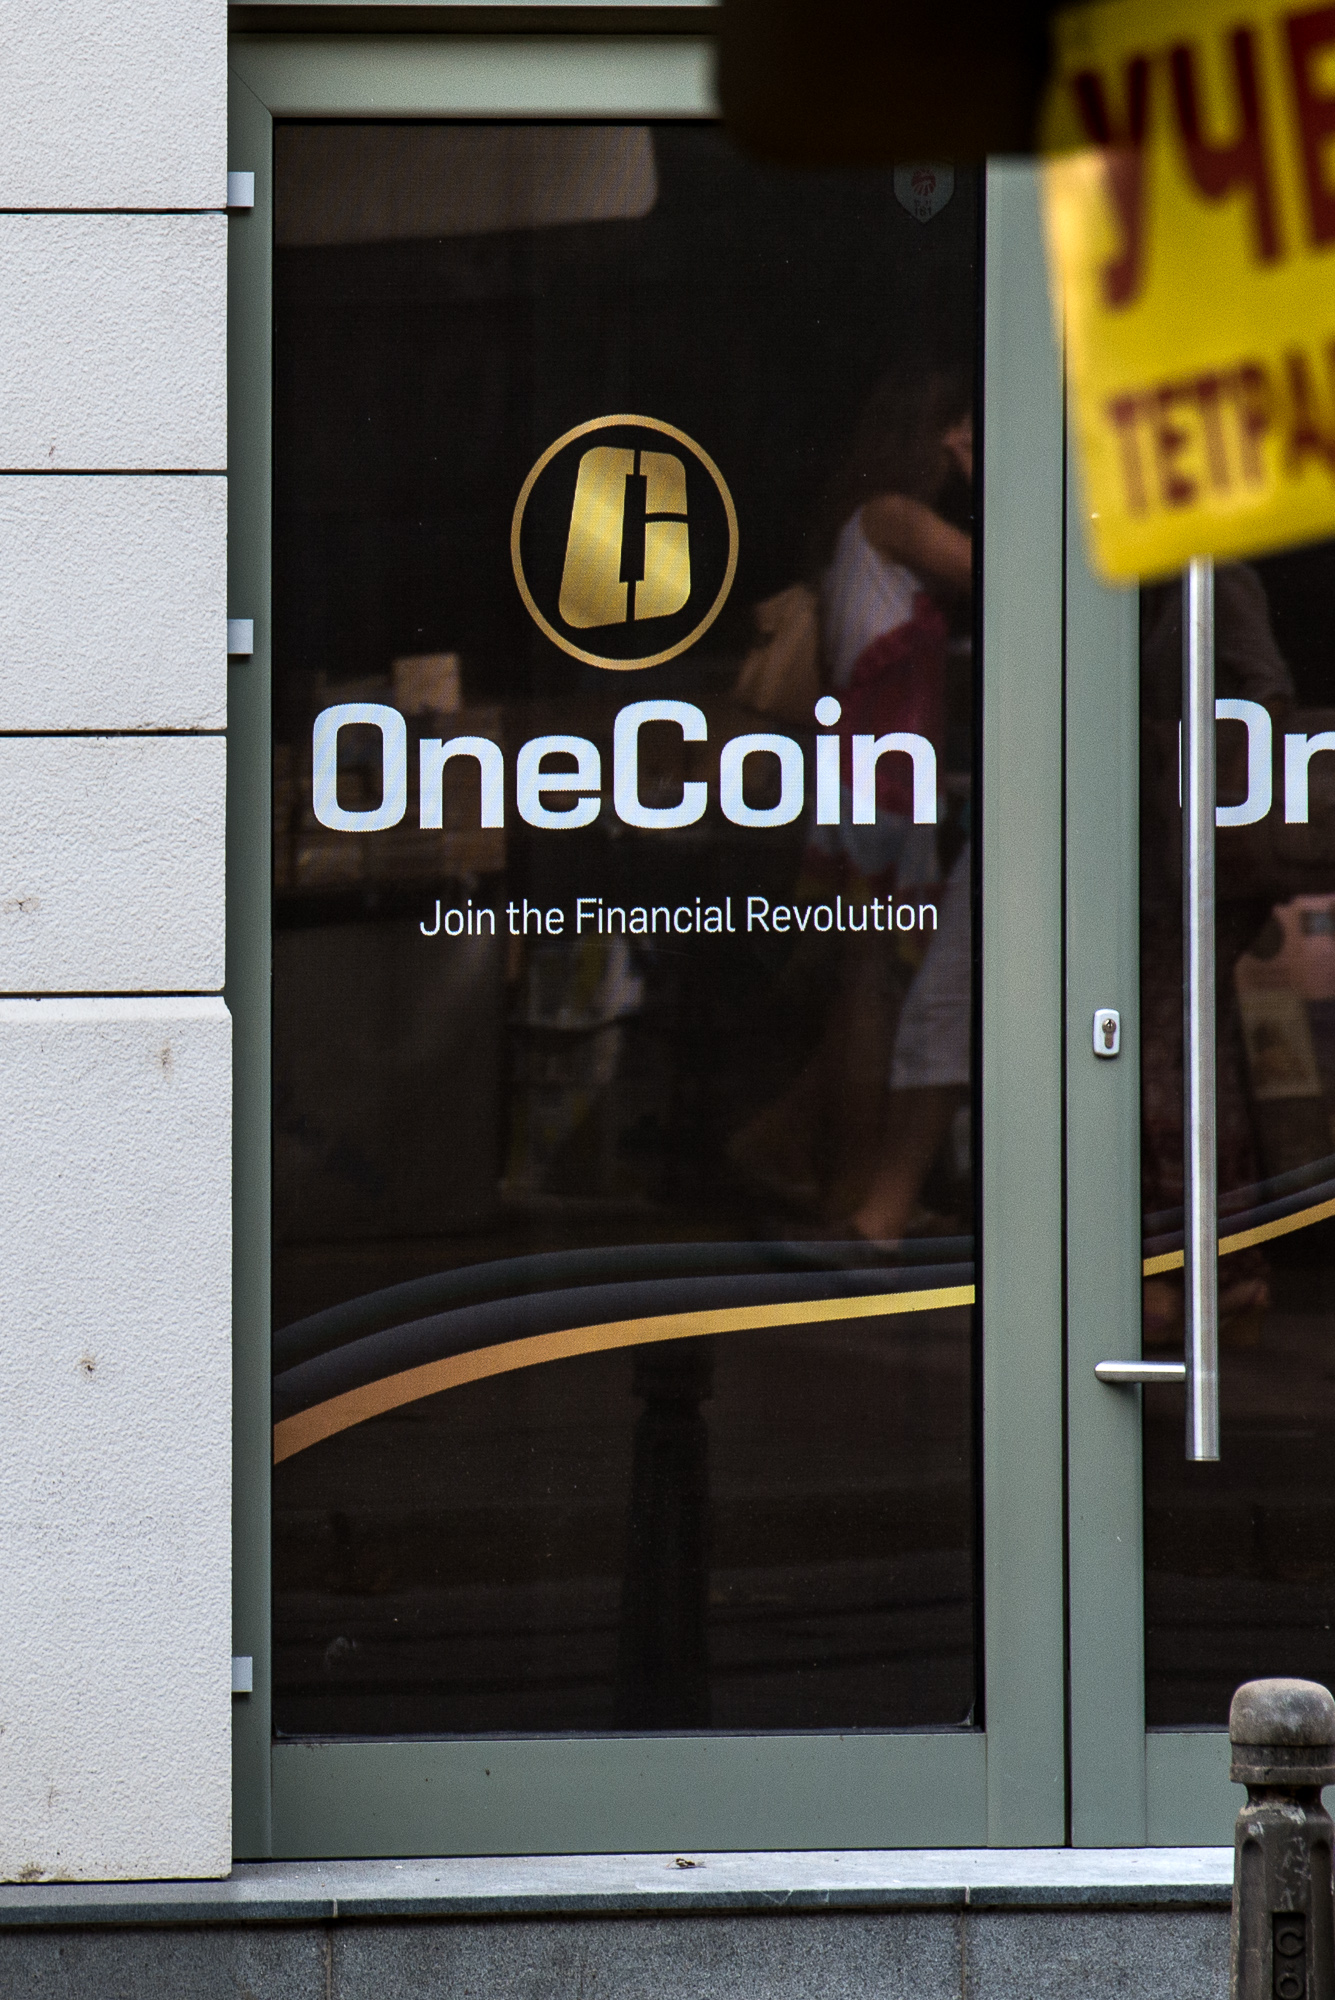
\includegraphics[width=0.4\textwidth]{imagens/onecoin.jpg}}
    \caption{Estabelecimento da OneCoin}
    \label{onecoin}
\end{figure}
\\
\\
\\   %organização
\\
Com tanto lucro, era muitas vezes vista a frequentar os mais ricos locais. Porém, ao contrário do caso de Maksim, tratado acima, Ignatova não conseguiu viver em legítima liberdade depois deste esquema. A OneCoin foi investigada e descobriram tudo. O dinheiro era feito pela angariação de novos clientes, e não pela valorização da moeda, tal como qualquer esquema em pirâmide. Assim, em janeiro de 2017, a plataforma foi encerrada.Com as buscas, em outubro de 2017, Ignatova fugiu para Atenas e nunca mais foi encontrada. Diz-se que a mesma fez uma cirurgia plástica de modo a passar despercebida nas ruas e complicar a descoberta do seu paradeiro \cite{osmaisprocurados}.  
\\ \indent Atualmente, é a única pessoa diretamente relacionada com a OneCoin que ainda não foi presa. O cofundador, Sebastian Greenwood foi preso com 20 anos de prisão, e o irmão da mesma, Konstantin Ignatov, foi preso também, porém já se encontra em liberdade, depois de 34 meses atrás das grades pois o mesmo concordou com 2 anos sob supervisão judicial e devolveu 118 mil euros dos fundos que conseguiu ao trabalhar na OneCoin. A rainha das criptomoedas continua em liberdade e tornou-se parte dos 10 mais procurados do \ac{fbi} \cite{fbi}. 

\section{Os Hackers da Coreia da Norte}
A Coreia do Norte começou a investir desde muito cedo em ciber operações, roubando milhões de dólares a bancos, crypto e companhias, o que atraiu a atenção global. Dois dos mais famosos são:

\begin{itemize}

\item{o \textit{hack} da Sony Pictures em 2014}
\item{o banco do Bangladesh em 2016}

\end{itemize}

Este tipo de operações, que necessitam de muito pouco investimento e têm grande recompensa permitiram ao governo de se estabelecer e se financiar. Os hackers da Coreia do Norte são estritamente treinados e monitorizados para prevenir a sua lealdade sendo um dos departamentos mais secretos e restritos do país. Estas operações são normalmente realizadas pelo grupo Lazarus que treina hackers do mais alto nível, envolvidos em diversas operações a escala mundial. Com o crescimento deste grupo, o investimento em cibersegurança subiu drasticamente, especialmente depois do ataque ao governo da Coreia do Sul, que custou milhões de dólares a este \cite{coreia}. 

\begin{figure}[h]
    \center
    \fbox{
\includegraphics[width=0.5\textwidth]{imagens/lazarus.png}}
    \caption{Lazarus}
    \label{lazarus}
\end{figure}

A história de Jong Yuli começa numa pequena cidade da Coreia do Norte, um país em que o estatuto social e as oportunidades de vida estão fortemente dependentes da família em que nasceste e o seu status. Jong nasceu numa família relativamente boa, dando-lhe espaço para se focar nos estudos. Desde muito pequeno que tinha um talento especial com números e seu pai deciciu investir nesse talento, o que o levou mais tarde a ser selecionado para as olimpíadas \ac{oim}. Devido ao facto da Coreia do Norte levar as competições muito mais a sério, Jong passou por uma preparação muito rigorosa, passando horas a resolver problemas complexos que não só tem o objetivo de melhorar as suas capacidades matemáticas, mas também o seu senso de patriotismo e dever para com o país.\\ \indent Depois da sua primeira saída do país para as \ac{oim} em Colômbia, Jong apenas obteu a medalha de prata e não a de ouro, o que levou ao descontentamento do regime já que tinham investido muito para o treino dele, esperando que este ganhasse o ouro. Yuli começou a perguntar-se o porquê de o seu país investir tanto em jovens como ele, e a perguntar-se sobre os seus objetivos, descobrindo através de um amigo que o governo estava a interrogar a sua família e a prepararem-se para o treinarem para ser um hacker.\\ \indent Jong percebeu que se fosse selecionado não teria o direito de recusar, e que viveria num regime restrito e afastado da sociedade. Como tinha até aos 18 anos para participar nas olimpíadas, percebeu que a sua última oportunidade para escapar do país seria em 2016. Depois de ganhar prata novamente, Jong aproveitou a chance e entrou em contacto com diplomatas da Coreia do Sul, que negociaram pacificamente a sua saída. Nos 2 anos que se seguiram a Coreia do Norte suspendeu a sua participação nas Olimpíadas e devido a este incidente, os participantes são acompanhados por um agente, para impedir que escapem.\\ \indent Jong vive agora na Coreia do Sul sob outro nome, tendo estudado Matemática na universidade. Ele nunca mais viu os pais desde que escapou.

\section{O rapaz que hackeou a \ac{nasa}}
\ac{nasa}, o sistema mais seguro do mundo, invadido por um rapaz de 15 anos. Jonathan James foi um \textit{hacker} dos \ac{eua}. Foi a primeira pessoa a ser presa por um cibercrime na América com 16 anos no ano 2000, um ano depois de cometer o seu maior crime cibernético: Invadir a \ac{nasa}. \\
\begin{figure}[h!]
    \center
    \fbox{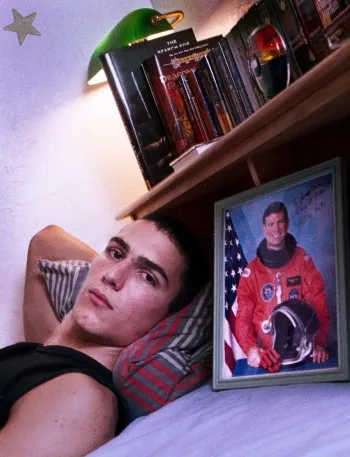
\includegraphics[width=0.3\textwidth]{imagens/jonathanjames.png}}
    \caption{Jonathan James}
    \label{jonathanjames}
\end{figure}
\\
Como qualquer criança, James jogava horas a fio no computador, ainda mais por o ser pai ser programador e o computador estar muito presente na sua vida. O problema começou quando o mesmo se começou a interessar mais em como o computador funcionava do que nos jogos. Numa entrevista em 1990, o pai de Jonathan disse que um dia chegou a casa e o filho tinha substituido o Windows pelo o Linux, num tempo em que o conhecimento tecnológico não era nem metade do que é hoje. \\ \indent A partir daí, foi-se interessando cada vez na arte da programação, e por diversão, invadia vários servidores. Em junho de 1999, Jonathan encontrou um servidor com uma segurança vulnerável em Alabama, o mesmo plantou um malware e ganhou o controlo de 13 outros computadores no sistema. James depois reparou que conseguiu acesso ao Marshall Space Flight Center, em Huntsville, uma unidade que trabalha em desenvolver foguetes e mantinha comunicações com a Estação Internacional do Espaço. Conseguiu roubar 1,7 milhões de euros em textit{data}. Foi depois revelado que muita da informação roubada era o código fonte para um software que controlava a temperatura e humidade do espaço vital da \ac{eei}, elementos vitais para a sobrevivência. Quando a \ac{nasa} reparou na quebra de segurança, fecharam a rede por 21 dias, resultando em 41 mil euros de perda \cite{desconhecido}. 
\\
\begin{figure}[h]
\begin{minipage}{0.45\textwidth}
    \center
    \fbox{
\includegraphics[width=0.8\textwidth]{imagens/nasa.jpg}}
    \caption{NASA}
    \label{nasa}
\end{minipage}
\begin{minipage}{0.45\textwidth}
    \center	
    \fbox{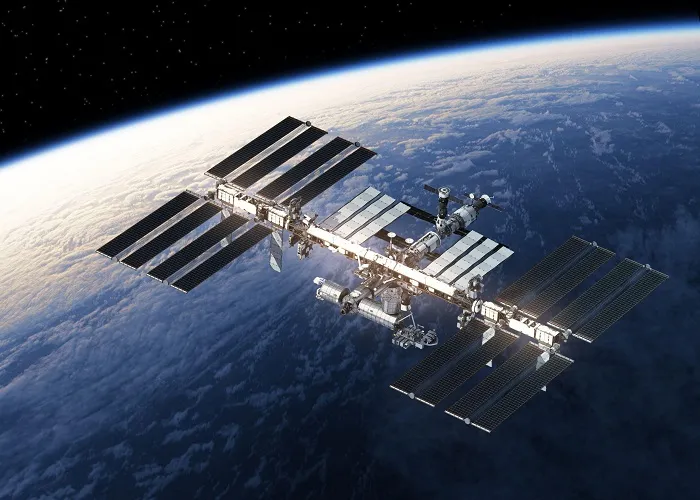
\includegraphics[width=0.8\textwidth]{imagens/eei.png}}
    \caption{Estação Espacial Internacional}
    \label{eei}
\end{minipage}
\end{figure}
\\ \indent Daí adiante, o \ac{fbi} focou-se em encontrar Jonathan. Tal aconteceu no dia 26 de janeiro de 2000. Como Jonathan tinha apenas 16 anos, acabou por ser sentenciado com 6 meses de prisão domeciliária e com uma proibição de uso do computador para qualquer outro assunto sem ser estudos. Para além disso, teve de escrever uma carta de desculpas para as empresas atacadas pelo mesmo, entre elas a \ac{nasa}. Também teve de trabalhar para as mesmas ao mostrar exatamente como conseguiu aceder aos sistemas. Mais tarde, Jonathan desrespeitou as regras e foi apanhado drogado na rua. Por essa razão, foi mandado para uma prisão juvenil em Alabama, onde permaneceu 6 meses. \cite{jonathanjames} \\ \indent Tempos depois de regressar a casa, em janeiro de 2008, foi desmascarado um virus e deduziram que James fez parte do mesmo por haver várias menções de um "JJ" e por ser amigo do lider desse ataque. Jonathan negou todas as alegações. Porém, mesmo assim, a polícia decidiu investigar a sua casa. Acabaram por não encontrar nada que ligasse Jonathan James e o virus, mas encontraram uma pistola e uma carta de suícidio e mesmo assim, não desistiram da especulação. Duas semanas depois, Jonathan foi encontrado morto em casa, com uma carta ao lado, escrito: "(...) Eu não acredito no sistema da "justiça". Talvez as minhas ações hoje, juntamente com esta carta, transmitam às pessoas uma mensagem mais forte. De qualquer das formas, perdi o controlo desta situação, e esta é a única maneira de consegui-lo de volta.(...)" de acordo com Daily Mail \cite{osmaisnotaveis}. Mais tarde foi descoberto que "JJ" era de Jim Jones, apelido de Stephen Huntley Watt.

\chapter{A Solução}

%%%%%%%%%%%%%%%%%%%%%%%%%%%%%%%%%%%%%%%%%%%%%%%%%%%%%%%%%%%%%%%%%%%%%%%%%%%%%%%%%%%%%%%%%%%%

\label{chap.a-solução}
\section{A importância da Cibersegurança}
Tal como referimos no \autoref{chap.introducao}, a cibersegurança é um tópico de cada vez mais importância na sociedade atual, uma sociedade em que há cerca de 4000 ciberataques por segundo, e mais de 600 milhões de ataques por dia \cite{ataques}. Uma das razões pelas quais este tipo de crime continua a aumentar é porque é barato, rápido e com uma alta recompensa e menos risco de ser apanhado, se comparado a outros tipo de crime. \\ \indent Cibercrimes podem custar milhões às empresas em termos de danos, como visto no \autoref{chap.os-crimes} e não estamos a falar apenas de dinheiro, mas da credibilidade da mesma, a sua capacidade de fazer negócios bem como a segurança dos seus trabalhadores e afiliados. A cibersegurança é muito importante pois mantém os dados dos seus clientes privados e a salvo, dando-lhes a confiança necessária na marca utilizada.
É importante que todas as empresas e indivíduos deem atenção à cibersegurança já que algmas instituições dependem de sistemas digitais para operar. Isto significa que uma violação de segurança pode causar interrupções afetando a receita da empresa, e em casos mais extremos a falência desta.
\section{A evolução dos Ciberataques e da Cibersegurança}

Como é possível ver acima, a cibersegurança é \textbf{muito importante} e por isso mesmo, é importante que a mesma evolua. Mas será que a mesma está a crescer da mesma forma que o uso da internet cresce atualmente?
\\ \indent Analisando os gráficos da \autoref{1}, da \autoref{2} e da \autoref{3}, é possível verificar a quantidade de quebras de informação por indústria para diferentes anos. No ano de 2022, houve um pico de 973 quebras de informação em agosto, no ano de 2023, um pico de 1151 em setembro e, agora em 2024, o máximo obtido foi de 525  em janeiro, até onde se sabe.
Dentro disto, o ano de 2024 parece o mais controlado e com menos quebras de informação. \\ \indent

\begin{figure}[h!]
    \centering
    \begin{tikzpicture}
        \begin{axis}[
            width=10cm,
            height=5cm,
            ybar stacked,
            bar width=15pt,
            ylabel={Quebras de Informação},
            xlabel={Meses},
            symbolic x coords={1,2,3,4,5,6,7,8,9,10,11,12},
            xtick=data
        ]
            \addplot [fill=red] coordinates {(1,259) (2,126) (3,174) (4, 143) (5,214) (6,351) (7,531) (8,973) (9, 258) (10, 197) (11, 219) (12, 134)};
            
            \addlegendentry{2022}
            \end{axis}
    \end{tikzpicture}
    \caption{Quebras de informação em 2022, Fonte: Identity Theft \cite{crimesciberneticos}}
    \label{1}
    \begin{tikzpicture}
        \begin{axis}[
            width=10cm,
            height=5cm,
            ybar stacked,
            bar width=15pt,
            ylabel={Quebras de Informação},
            xlabel={Meses},
            symbolic x coords={1,2,3,4,5,6,7,8,9,10,11,12},
            xtick=data
        ]
            \addplot [fill=orange] coordinates {(1, 202) (2, 128) (3, 251) (4, 285) (5, 467) (6, 534) (7, 376) (8, 537) (9, 1151) (10, 772) (11, 875) (12, 316)};
           	\addlegendentry{2023}
            
             \end{axis}
    \end{tikzpicture}
    \caption{Quebras de informação em 2023, Fonte: Identity Theft \cite{crimesciberneticos}}
    \label{2}
    \begin{tikzpicture}
        \begin{axis}[
            width=10cm,
            height=5cm,
            ybar stacked,
            bar width=10pt,
            ylabel={Quebras de Informação},
            xlabel={Meses},
            symbolic x coords={1,2,3,4,5,6,7,8,9,10,11},
            xtick=data
        ]
            \addplot [fill=pink] coordinates {(1,525) (2, 368) (3, 366) (4, 452) (5, 245) (6, 259) (7, 190) (8, 312) (9, 261) (10, 339) (11, 285)};
           	\addlegendentry{2024}
            
             \end{axis}
    \end{tikzpicture}
    \caption{Quebras de informação em 2024, Fonte: Identity Theft \cite{crimesciberneticos}}
    \label{3}
\end{figure}
Dentro destes ataques existem vários tipos, na \autoref{tiposdeataques} é possível ver os mais utilizados em 2022: \\
\\
\\
\begin{figure}[h!]
    \begin{tikzpicture}
        \pie[text=legend, radius=3]{
            53.2/Phishing, 9.2/Compras sem entrega, 10.4/Roubo de Identidade, 27.2/Outros
        }
    \end{tikzpicture}
    \caption{Tipos de ataques em 2022, Fonte: Crimes cibernéticos \cite{estatistica}}
    \label{tiposdeataques}
\end{figure} \\

Como \textbf{ainda} não existe nenhum dado para este tema em 2024, só podemos deduzir que não tenha mudado muito. Porém, em 2017 houve também uma análise: \\
\begin{figure}[h!]
    \begin{tikzpicture}
        \pie[text=legend, radius=3]{
            12.5/Phishing, 41.6/Compras sem entrega, 8.7/Fraude financeira, 37.2/Outros
        }
    \end{tikzpicture}
    \caption{Tipos de ataques em 2017, Fonte: Crimes cibernéticos \cite{estatistica}}
    \label{tiposdeataques2}
\end{figure} \\
Comparando os dois, verifica-se um \textbf{grande aumento} no \textit{phising}, um aumento em roubos de identidade e uma diminuição de compras sem entrega. Mas, para analisar melhor estes dados, é importante ter uma noção de quantos ataques houve em cada ano. Em 2022 houve um aumento de 51\% em tentativas de ataque comparativamente ao ano de 2021. Esse aumento continua a ser revelado hoje em dia, havendo cada vez mais tentativas a cada ano que passa. E não só tentativas, de acordo com a Huawei, o número de ciberataques tem crescido 20\% a cada ano, causando, de acordo com a Cybersecurity Ventures, uma perda de quase 1 500 triliões euros \cite{exame}.
\\ \indent Com estes dados, conclui-se que a cibersegurança ainda tem muito espaço para evoluir e que se deve investir cada vez mais. Felizmente, com a Inteligência Artificial a crescer, a cibersegurança vai ganhar outros meios e pode vir a crescer exponencialmente. Até lá, simples conhecimentos sobre como navegar de forma segura na internet são fulcrais para os dias de hoje e podem salvar muita informação.


\chapter{Conclusões}
\label{chap.conclusão}
Como foi abordado, os ataques cibernéticos \textbf{não} vão parar de acontecer, pelo contrário, vão cada vez acontecer mais. As consequências destes ataques são grandes e, infelizmente, quando acontecem são difíceis de reverter. Por causa disso, é muito importante permanecer seguro na internet e caso possível, manter as outras pessoas seguras também. \\ \indent Com este relatório ganha-se uma noção diferente do que de facto são \textbf{ciberataques e a sua dimensão}. Fica-se a conhecer as inúmeras consequências que estes têm e o que conseguem causar. O \autoref{chap.os-crimes}, os crimes, aborda este tema de uma forma interessante e cativante onde mostra várias situações, todas elas diferentes, mas com o \textbf{mesmo intuito}, isto é, remeter o leitor para a \textbf{importância da cibersegurança}. No \autoref{chap.a-solução} aborda-se isso mesmo, agora de uma forma mais técnica e direta, porém visual, com a ajuda dos gráficos apresentados. Nestes gráficos estão dados importantes para perceber melhor como a cibersegurança e os ataques estão a evoluir.

\chapter*{Contribuições dos autores}
\ac{jg}:
\begin{itemize}
    \item{Escolha do tema e capítulos abordados}
    \item{Introdução}
    \item{Capítulos 2.1, 2.4 e 2.6}
    \item{Capítulo 3.2}
    \item{Capítulo 4}
    \item{Acrónimos}
    \item{Bibliografia}
\end{itemize}

\ac{ms}:
\begin{itemize}
    \item{Escolha do tema e capítulos abordados}
    \item{Introdução}
    \item  {Resumo}
    \item {Capítulos 2.2, 2.3 e 2.5 }
    \item {Capítulo 3.1}
\end{itemize}

\vspace{10pt}
Percentagem de contribuição de cada autor: \ac{jg} 65\%, \ac{ms} 35\%\\

\vspace{10pt}
\textbf{Repositório GitHub:} \repo

%%%%%%%%%%%%%%%%%%%%%%%%%%%%%%%%%
\chapter*{Acrónimos}
\begin{acronym}
\acro{ua}[UA]{Universidade de Aveiro}
\acro{leci}[LECI]{Licenciatura em Engenharia de Computadores e Informática}
\acro{jg}[JG]{Joana Gião}
\acro{ms}[MS]{Matilde Sanches}
\acro{nasa}[NASA]{The National Aeronautics and Space Administration}
\acro{cia}[CIA]{Central Intelligence Agency}
\acro{ach}[ACH]{Automated Clearing House}
\acro{eua}[EUA]{Estados Unidos da América}
\acro{nca}[NCA]{National Crime Agency}
\acro{fbi}[FBI]{Federal Bureau of Investigation}
\acro{eei}[EEI]{Estação Espacial Internacional}
\acro{oim}[OIM]{Olimpíadas Internacionais da Matemática}
\end{acronym}
%%%%%%%%%%%%%%%%%%%%%%%%%%%%%%%%%
\printbibliography
\end{document}